\documentclass[11pt]{beamer}
%\documentclass[11pt, aspectratio=169]{beamer}
\usepackage[utf8]{inputenc}
\usepackage[ngerman]{babel}
\usepackage{tikz}
\usetikzlibrary{shadows}
\usepackage{graphicx}
\usepackage[many]{tcolorbox}

\usetheme{TuDo}
\begin{document}
	\author{Michael R. und Timon S.}
	\title{Smart Mirror}
	%\subtitle{}
	\institute{TU Dortmund - Fakult\"at f\"ur Informatik}
	\date{\today}
	%\subject{}
	%\setbeamercovered{transparent}
	\titlegraphic{
		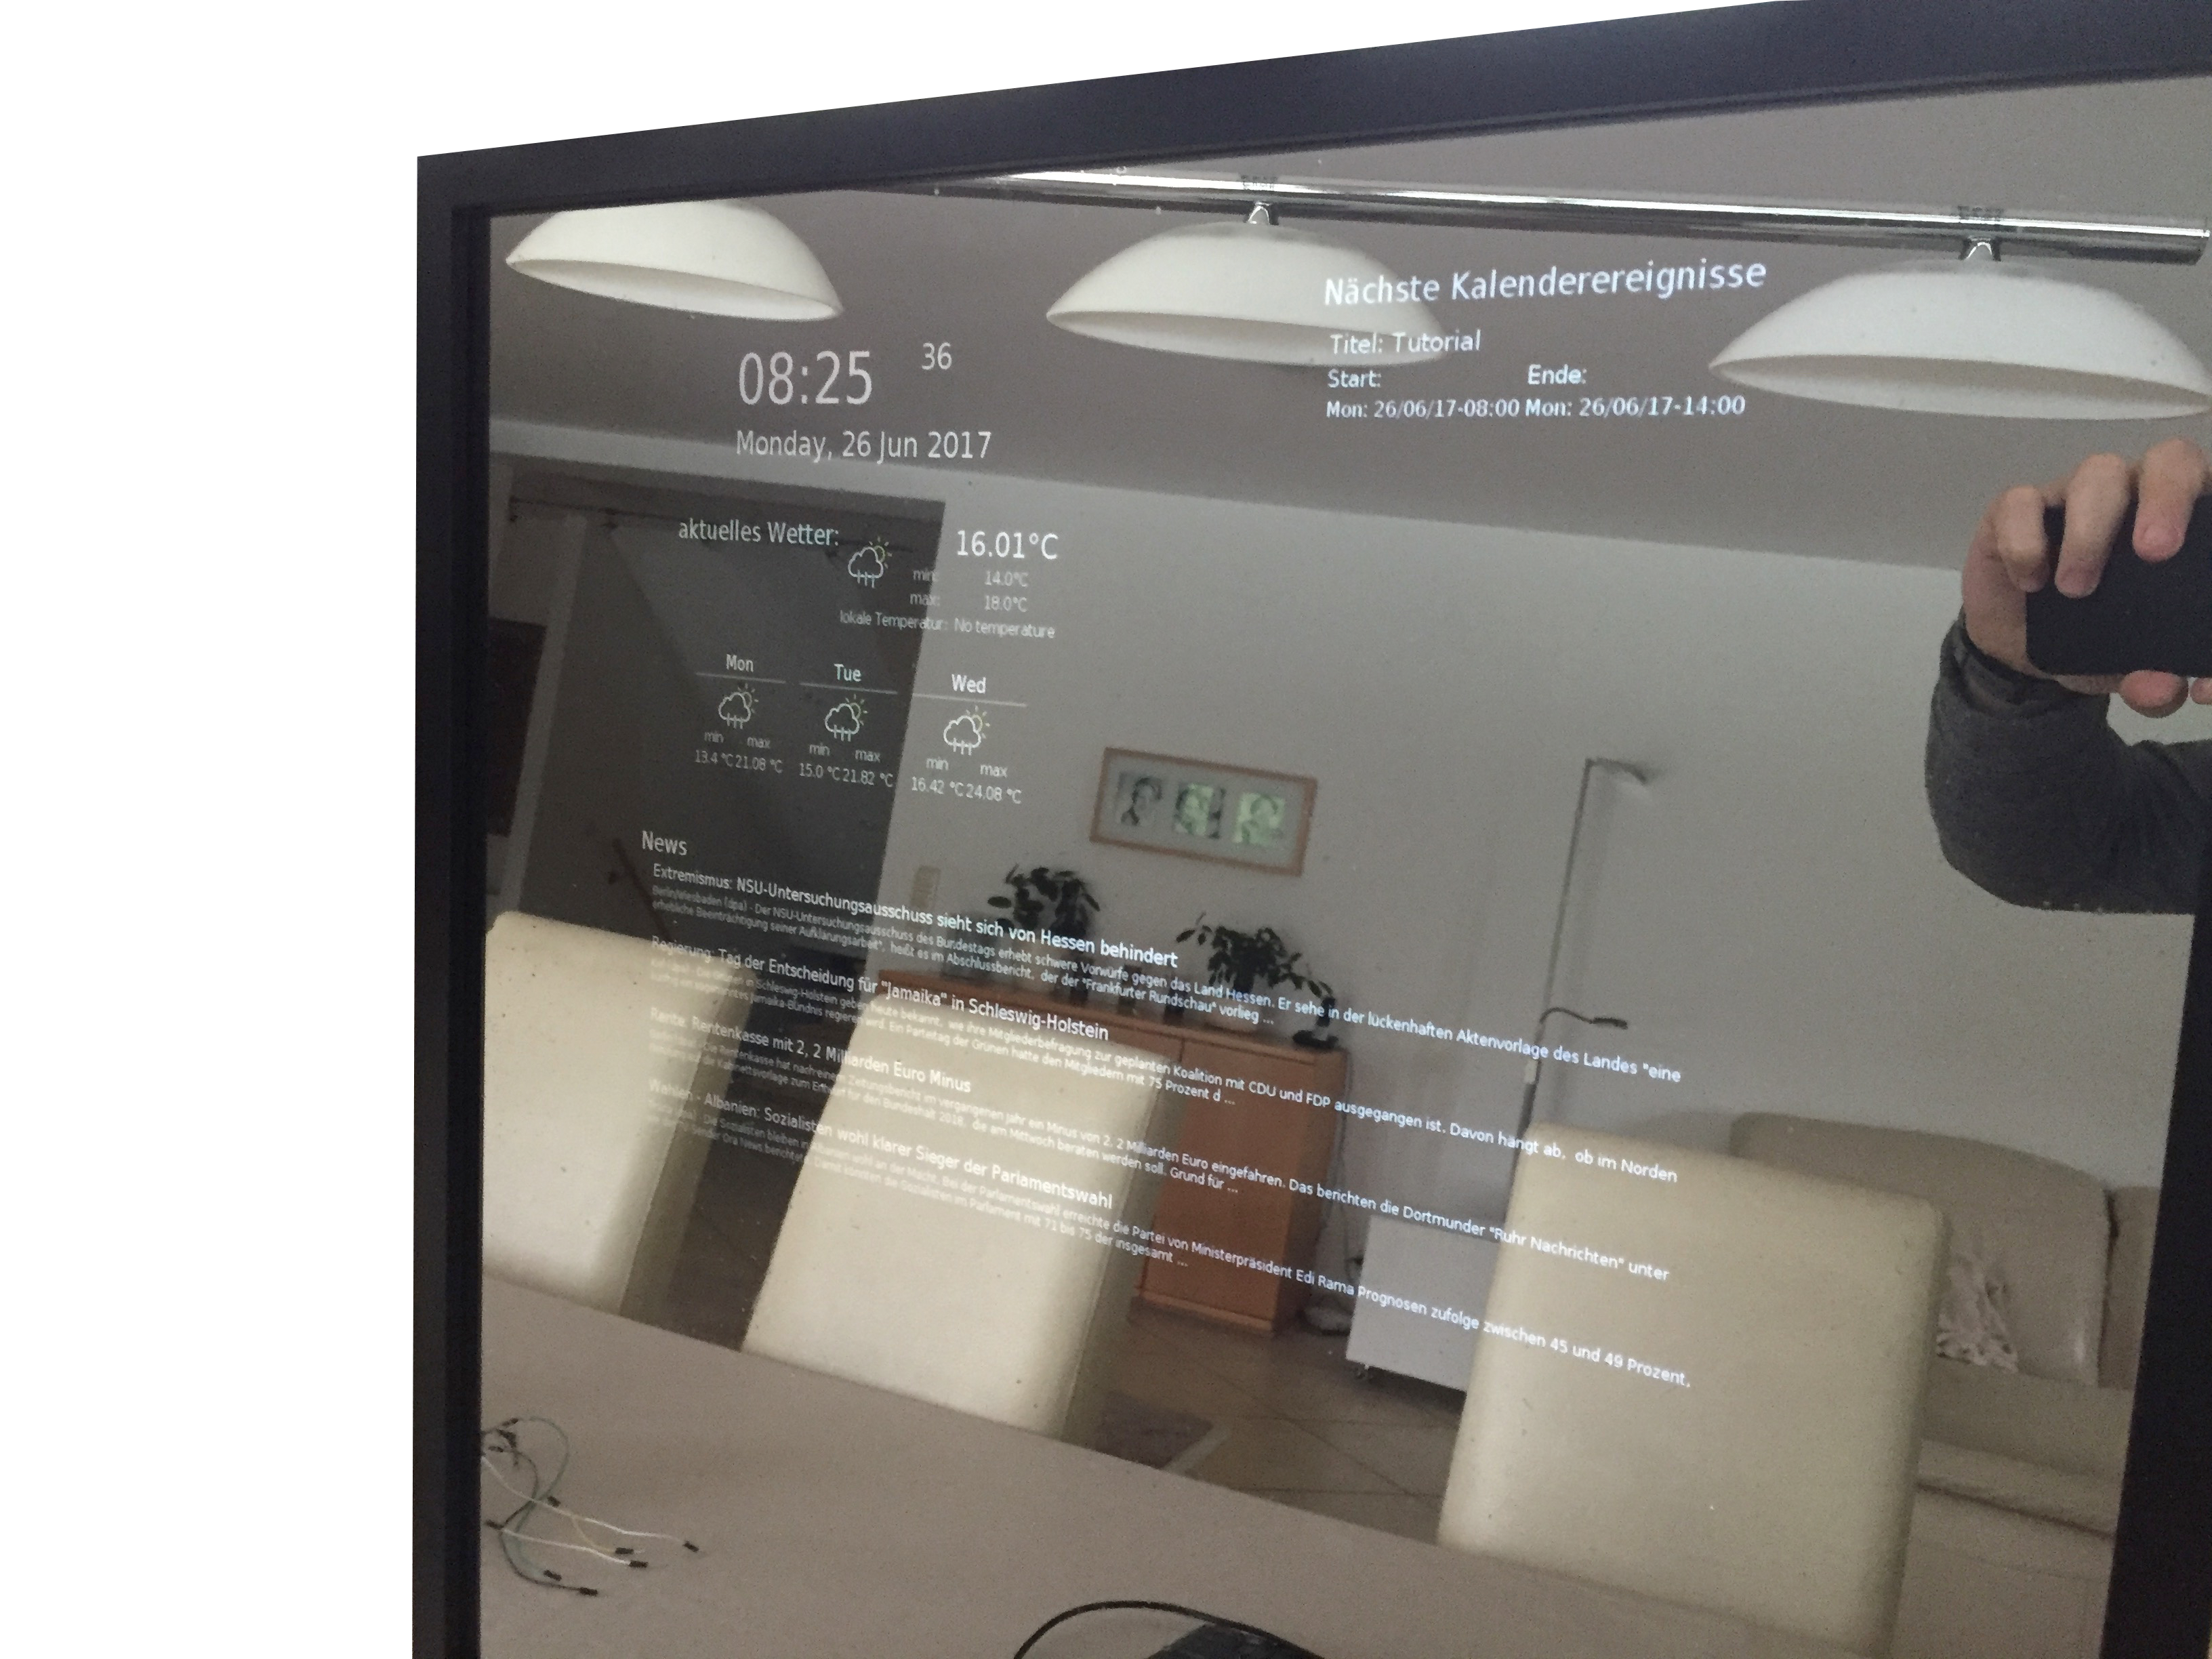
\includegraphics[width=0.35\paperwidth]{images/titlepage}
	}
	
	\begin{frame}
		\titlepage
	\end{frame}

	\begin{frame}
		\frametitle{Frage}
		\centering
		\huge
		\vfill
		Vergisst du auch h\"aufig den Geburtstag deiner Großeltern?
		\vfill
	\end{frame}

	\begin{frame}
		\frametitle{L\"osung}
		\centering
		\Large
		So kann dir das nicht mehr passieren!
		\includegraphics[width = .7\paperwidth]{images/showcaseImage}
	\end{frame}

	\begin{frame}
		\frametitle{Übersicht}
		\tableofcontents
	\end{frame}

	\section{Verteilung der Aufgaben}
	\begin{frame}
		\frametitle{Verteilung der Aufgaben}
	\end{frame}

	\section{technische Komponenten}
	\begin{frame}
		\frametitle{technische Komponenten}
	\end{frame}	

	\begin{frame}
		\frametitle{technische Komponenten}
	\end{frame}

	\subsection{Verteilungsdiagramm}
	\begin{frame}
		\frametitle{Verteilungsdiagramm}
	\end{frame}

	\section{UI}
	\begin{frame}
		\frametitle{Graphische Oberfl\"ache}
	\end{frame}
		
	\section{Programmierung}
	\subsection{Integration des MVC-Patterns}
	\begin{frame}
		\frametitle{Projektstruktur}
	\end{frame}

	\subsection{genutzte API's}
	\begin{frame}
		\frametitle{genutzte API's}
	\end{frame}

	
	\section{Fazit}
	\begin{frame}
		\frametitle{Fazit}
	\end{frame}
\end{document}